\documentclass[]{standalone}
\usepackage{tikz}
\begin{document}
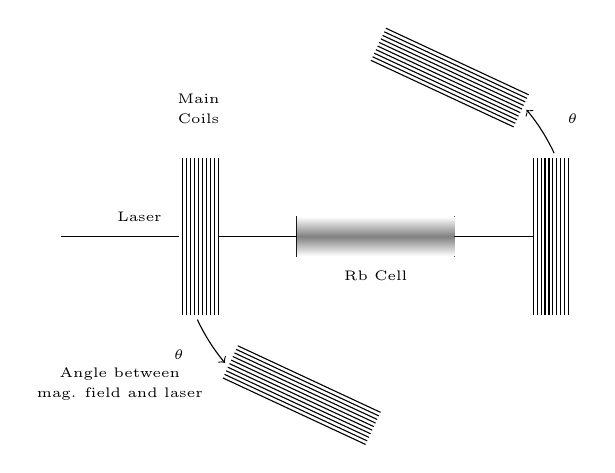
\begin{tikzpicture}
	\foreach \index in {0,.05,...,.5}
	{
		\draw (2+\index,1) -- (2+\index,-1);
		\draw (-2-\index,1) -- (-2-\index,-1);
	}
	\foreach \index in {0,.05,...,.5}
	{
		\draw[rotate = 65] (2+\index,1) -- (2+\index,-1);
		\draw[rotate = 65] (-2-\index,1) -- (-2-\index,-1);
	}
	\draw (-1,-.25) rectangle +(2,+.5);
	\shade[bottom color = white, top color = gray] (-1,0) rectangle (1,-.25);
	\shade[top color = white, bottom color = gray] (-1,0) rectangle (1,.25);
	\node at (0,-.5) {\tiny Rb Cell};
	\node at (-2.25,1.75) {\tiny Main};
	\node at (-2.25,1.5) {\tiny Coils};
	\node at (-3,.25) {\tiny Laser};
	\node at (-2.5,-1.5) {\tiny $\theta$};
	\node at (2.5,1.5) {\tiny $\theta$};
	\node at (-3.25,-1.75) {\tiny Angle between};
	\node at (-3.25,-2) {\tiny mag. field and laser};
	\draw (-4,0) -- (-2.5,0);
	\draw (-2,0) -- (-1,0);
	\draw (1,0) -- (2,0);

	\draw[->] (205: 2.5cm) arc (205:220:2.5cm);
	\draw[->] (25: 2.5cm) arc (25:40:2.5cm);


\end{tikzpicture}



\end{document}
